\section{视网膜的显微解剖}
\begin{frame}
    \frametitle{视网膜结构}

    \begin{columns}
        \column{0.5\textwidth}{
        下面介绍光能转化为神经活动的过程。先介绍视网膜细胞结构,
        以便大致了解图像处理过程。

        如图\ref{pic4-1},光信息自色素吸收后通过光感受器经双极细胞传导至神经节细胞,
        神经节细胞的轴突汇聚成视神经离开眼球。水平细胞和无长突细胞通过侧向联系调节双极细胞和神经节细胞。
        }
        \column{0.5\textwidth}{
            \begin{figure}
                \centering
                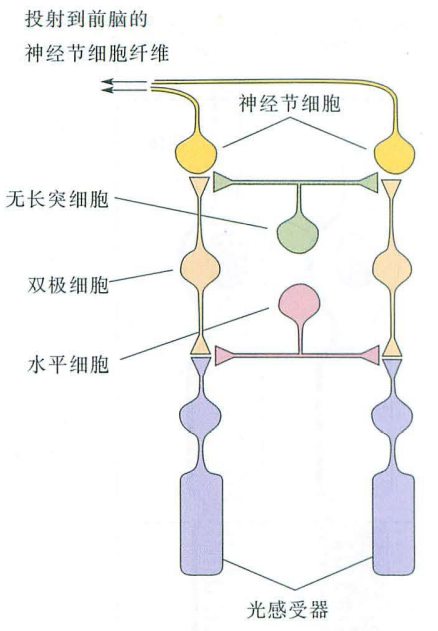
\includegraphics[width=0.6\textwidth]{img/pic4-1.png}

                \caption[]{{视网膜信息处理系统}\label{pic4-1}}
            \end{figure}
        }
    \end{columns}

\end{frame}
\subsection{视网膜的分层组构}
\begin{frame}
    \frametitle{视网膜分层组构}

    \begin{columns}
        \column{.5\textwidth}{
            注意到,光必须穿过几个细胞层才能到达位于视网膜后端的光感受器细胞。视网膜按相对眼球中央的位置由里到外命名:
            \scriptsize{
            \begin{itemize}
                \item \textbf{神经节细胞层}(ganglion cell layer),包含神经节细胞的胞体
                \item \textbf{内核层}(inner nuclear layer),含有双极细胞,水平细胞和无长突细胞的胞体
                \item \textbf{外核层}(outer nuclear layer),含有光感受器胞体
                \item \textbf{光感受器外段层}(layer of photoreceptor outer segments)
            \end{itemize}
            }
        }
        \column{.5\textwidth}{
            \begin{figure}
                \centering
                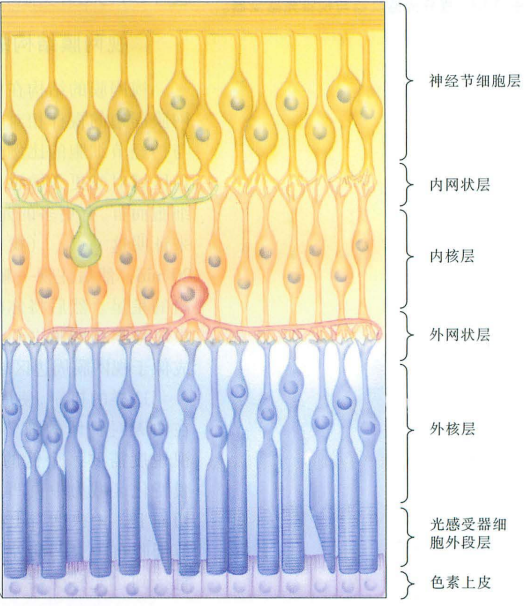
\includegraphics[height=.7\textheight]{img/pic4-2.png}
                \caption{视网膜的分层组构\label{pic4-2}}
            \end{figure}
        }
    \end{columns}

\end{frame}

\subsection{光感受器的结构}
\begin{frame}
    \frametitle{光感受器结构}

    \begin{columns}
        \column{.6\textwidth}{
            光辐射与神经信号的转换发生在视网膜后部的1.25亿个光感受器中。每个光感受器由外段、内段、胞体和突触终末组成。
            \textbf{外段}含有大量膜盘(membranous disk),其上存在光敏感的视色素对光进行吸收,触发光感受器膜电位的变化。
            根据外段外形不同分为:
            \scriptsize{
                \begin{itemize}
                    \item \textbf{视杆光感受器}(rod photorecptor):具有较长的桶状外段,其中含有大量膜盘,不同视杆色素无差异
                    \item \textbf{视锥光感受器}(cone photorecptor):具有较短锥形外段,含有膜盘数较少但色素密度高且存在三种色素类型
                \end{itemize}
            }
            这导致了视网膜的双重性:暗视视网膜只是用视杆,明视视网膜主要使用视锥。视色素差异导致各种视锥对不同波长的光敏感,即仅由视锥对色觉有贡献。
        }
        \column{.4\textwidth}{
            \begin{figure}
                \centering
                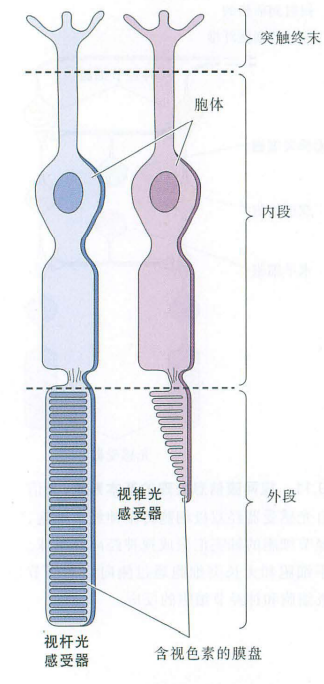
\includegraphics[width=.5\textwidth]{img/pic4-3.png}
                \caption{视杆与视锥光感受器\label{pic4-3}}
            \end{figure}
        }
    \end{columns}

\end{frame}


\subsection{视网膜结构的区域差异}

\begin{frame}
    \frametitle{视网膜结构的区域差异}
    
    \begin{columns}
        \column{.5\textwidth}{
            视网膜的结构在中央凹和视网膜的周边是有所不同的。其细胞分布如图\ref{pic4-4}(a),
            视锥主要集中在视网膜的中心,视杆细胞主要分布于周边视网膜,中央凹内没有视杆细胞。

            由结构图\ref{pic4-4}(b),在视网膜中心由较少的光感受器细胞直接向一个神经节细胞提供信息;在周边视网膜则较多。
            这一结构安排使得周边视网膜对暗淡光线的检测更为有利,而中心视网膜则对提高视觉精度更为有利。
        }
        \column{.5\textwidth}{
            \begin{figure}
                \centering
                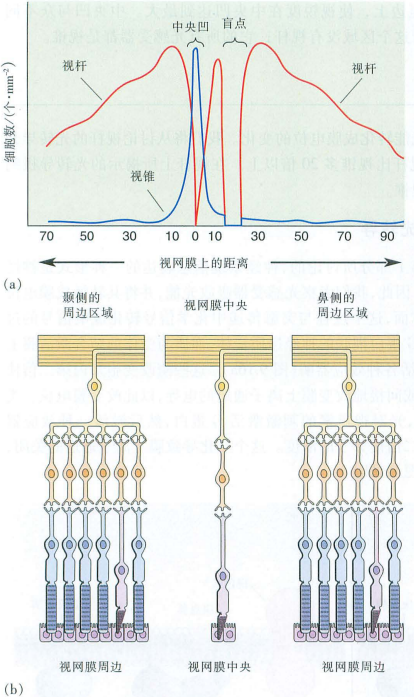
\includegraphics[height=.7\textheight]{img/pic4-4.png}
                \caption{视网膜细胞分布的区域差异\label{pic4-4}}
            \end{figure}
        }
    \end{columns}

\end{frame}
\begin{frame}
    \frametitle{视网体结构汇总}
    \begin{figure}
        \centering
        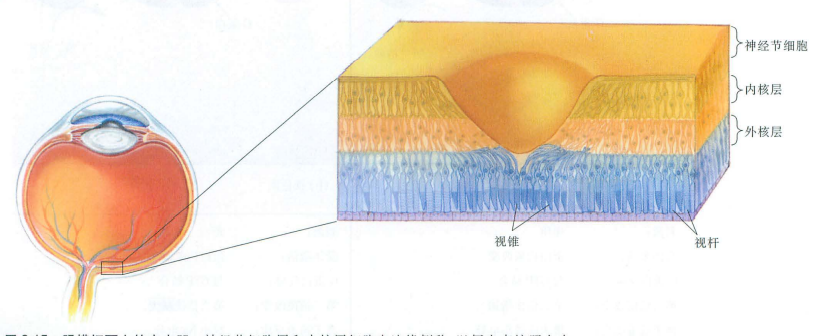
\includegraphics[width=.8\textwidth]{img/pic4-5.png}
        \caption{视网膜显微结构\label{pic4-5}}
    \end{figure}
    \tiny{Tip:图中神经节细胞层和内核层细胞向边缘侧移,以便光直接照在中央凹的光感受器上,提高中央区域的视锐度,同时也提升了周边视网膜的光敏感性。}

\end{frame}
